\begin{figure}[ht]
    \centering
    \resizebox{0.8\columnwidth}{!}{
        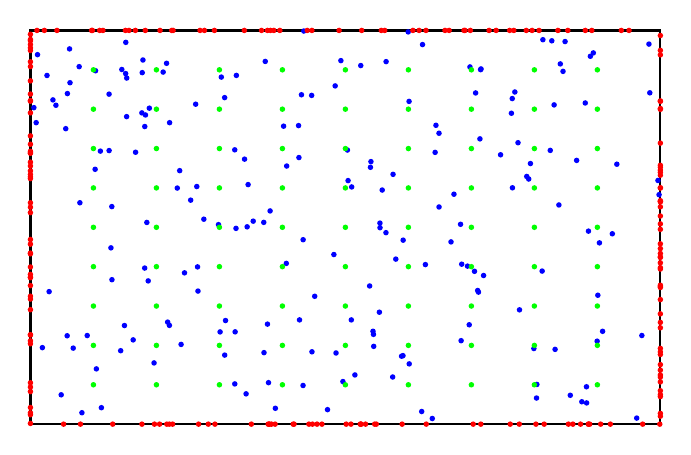
\begin{tikzpicture}
            % Прямоугольник  (размеры 8x5)
            \draw[thick] (-4,-2.5) rectangle (4,2.5);

            % Случайные точки внутри прямоугольника
            \foreach \i in {1,...,200} {
                \fill[blue] (rand*4, rand*2.5) circle (1pt);
            }

            % Случайные точки на гранях прямоугольника
            \foreach \i in {1,...,50} {
                % Нижняя грань
                \fill[red] (rand*4, -2.5) circle (1pt);
                % Верхняя грань
                \fill[red] (rand*4, 2.5) circle (1pt);
                % Левая грань
                \fill[red] (-4, rand*2.5) circle (1pt);
                % Правая грань
                \fill[red] (4, rand*2.5) circle (1pt);
            }

            \foreach \i in {-4,...,4} {
                \foreach \j in {-4,...,4} {
                    \fill[green] (4 * \i / 5, 2.5  * \j / 5) circle (1pt);
                }
            }
        \end{tikzpicture}
        }
        \caption{Распределение точек в прямоугольной области для обучения, где красные точки ---
        точки на границе, синие точки --- внутри области, зеленые точки --- совпадают с сеткой
        точного решения}
        \label{fig:points}
    \end{figure}